\section{Results}
\label{sec:results}

\begin{figure}[b]
  \centering
  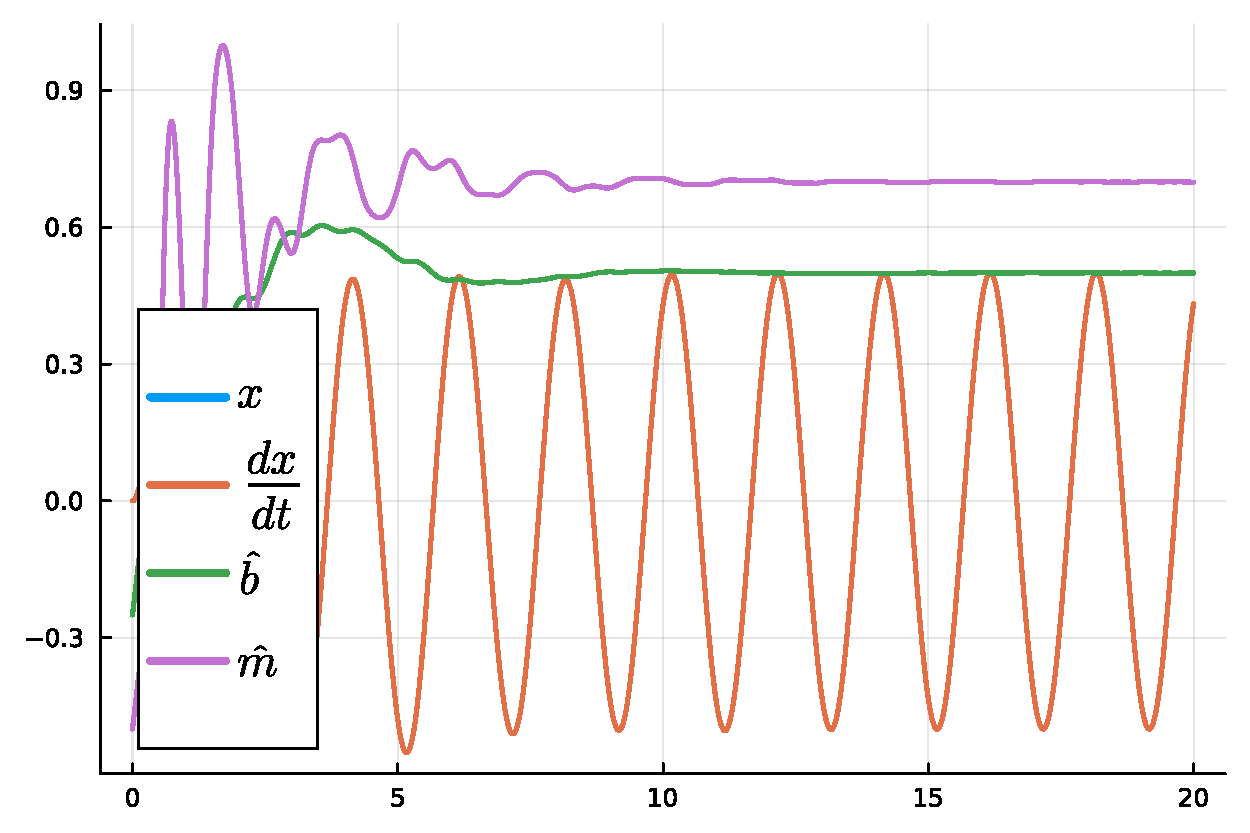
\includegraphics[width=0.5\textwidth]{./figures/adaptationrule1.pdf}
  \caption{Simulation showing the convergence of the system state and parameter
  estimates.}
  \label{fig:adaptation}
\end{figure}

\begin{figure}[b!]
  \centering
  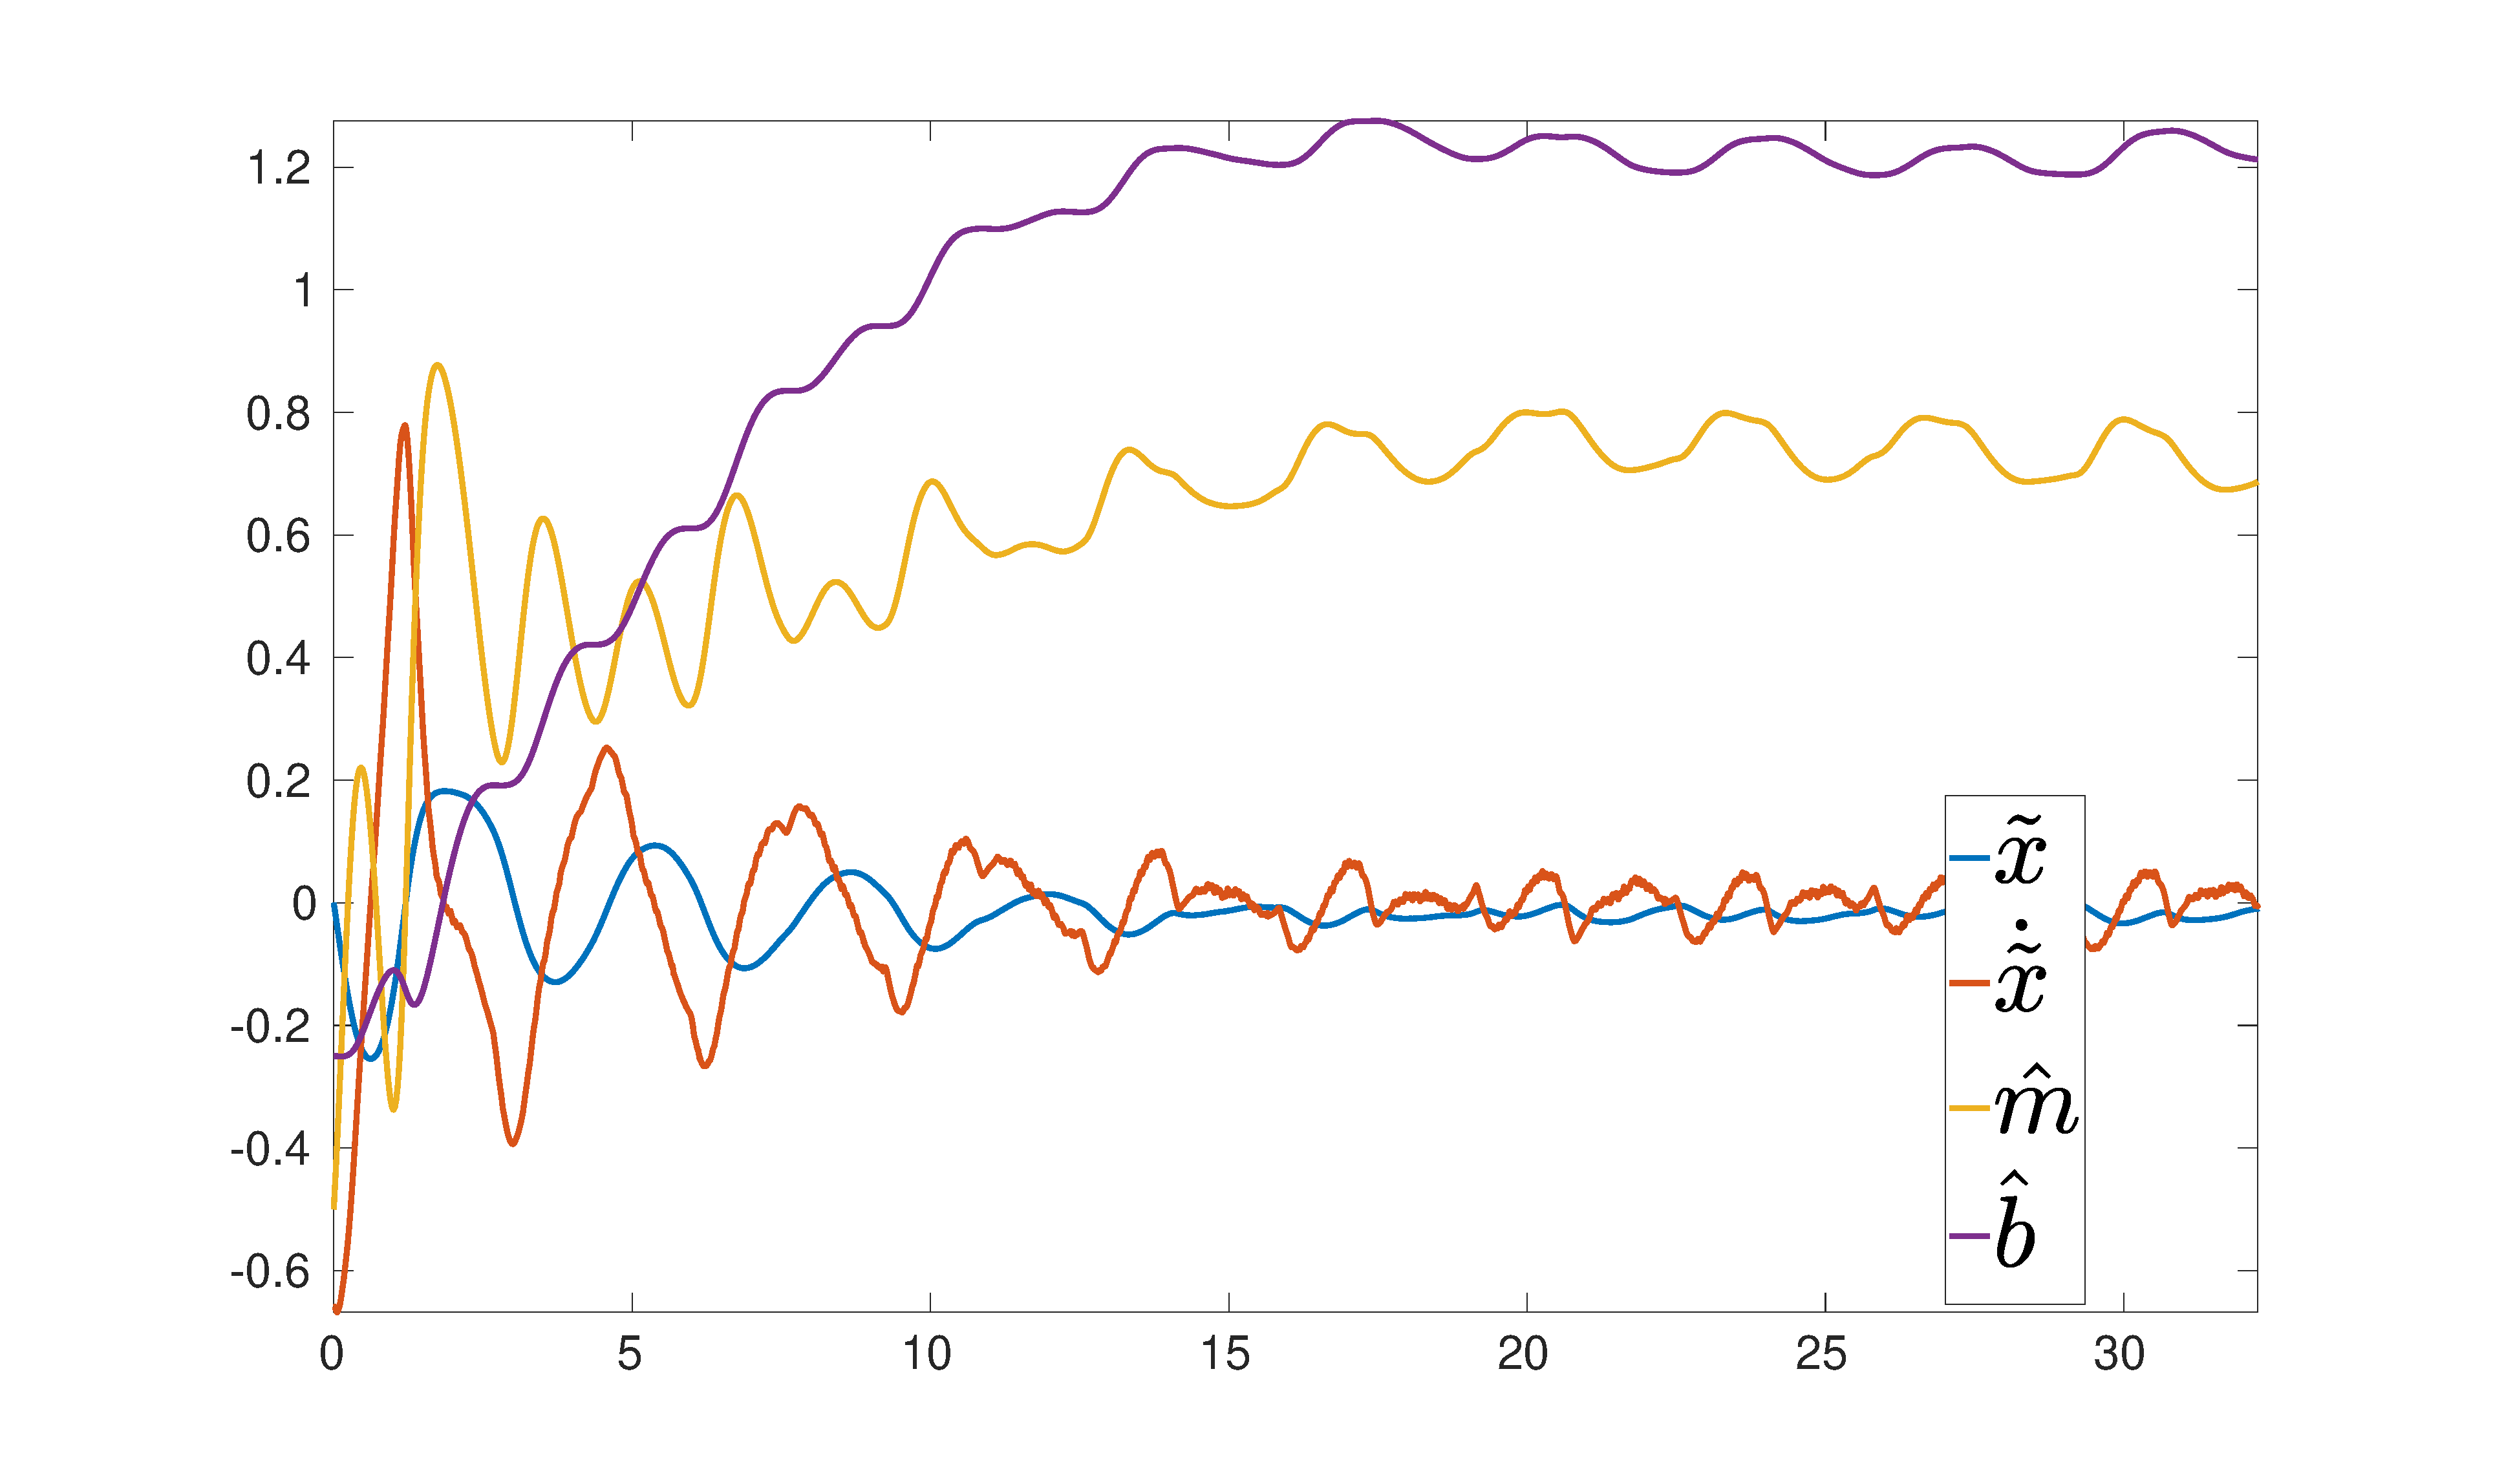
\includegraphics[width=0.5\textwidth]{./figures/station2_adaptation.eps}
  \caption{Hardware implementation of the estimation algorithm.}
  \label{fig:hardware}
\end{figure}

In Figure~\ref{fig:adaptation}, we plot the response of the system to the
control and adaptation laws~(\ref{eq:controller}, \ref{eq:adaptation}),
implemented in simulation. The constants that are used are as follows: $(A,
\omega, \varphi) = (\nicefrac{3}{10}, \nicefrac{3\pi}{5}, 0^\circ)$ and $(k,
\lambda) = (1, 4)$. The real mass and damping of the system is $(m, b) = (0.75,
1.22)$ and their estimates start at $(\hat{m}, \hat{b}) = (-\nicefrac{1}{2},
-\nicefrac{1}{4})$.

In Figure~\ref{fig:hardware}, we plot the response of the system to the control
and adaptation laws ~(\ref{eq:controller}, \ref{eq:adaptation}), implemented on
a real cart system. The constants used are as follows: $(A, \omega, \varphi) =
(\nicefrac{3}{10}, \nicefrac{3\pi}{5}, 0^\circ)$ and $(k, \lambda) = (1, 4)$. We
did not know the real mass and damping of the system and set our initial guesses
of them to be $(\hat{m}, \hat{b}) = (-\nicefrac{1}{2}, -\nicefrac{1}{4})$.

